\documentclass[journal]{IEEEtran}

\usepackage{amsmath,amsfonts}
\usepackage{algorithmic}
\usepackage{array}
\usepackage{booktabs}
\usepackage{cite}
\usepackage{graphicx}
\usepackage{multirow}
\usepackage{tikz}
\usepackage{xcolor}
\usepackage{xspace}
\usepackage{url}
\usetikzlibrary{arrows.meta,positioning}
\graphicspath{{figures/}}

\newcommand{\model}{DACP-Net\xspace}
\newcommand{\ap}{AP@[.50:.95]}
\newcommand{\pending}[1]{\textcolor{red}{[TBD: #1]}}

\begin{document}

\title{DACP-Net: Directional-Aware Content-Adaptive Pyramid Network for Closed-Loop Fabric Defect Inspection on Circular Knitting Machines}

\author{\pending{Author Name(s)}%
\thanks{\pending{Affiliation, city, country, and corresponding author information.}}%
}

\maketitle

\begin{abstract}
Continuous fabric inspection on circular knitting machines must recognize sparse, elongated defects under repetitive texture while responding quickly enough to support production intervention. This paper presents a closed-loop edge-cloud inspection workflow and DACP-Net, a lightweight detector tailored to this setting. In the workflow, a proximity-switch rotation signal enables inspection at the edge; the edge device acquires fabric images and issues a local stop command when a defect is detected. The candidate defect is then presented to an operator for confirmation, and both the detection and the confirmation are retained in the cloud for subsequent data curation and offline model improvement. DACP-Net starts from YOLOv8n and introduces a warp--weft texture encoding (WWTE) block that jointly models horizontal, vertical, and local texture responses, together with a local texture-guided feature reassembly (LTFR) block that replaces the two fixed top-down upsampling operations with content-adaptive reassembly. On a production-line dataset of 403 images covering horizontal defects, vertical defects, and holes, the retained test split contains 81 images and 91 instances. DACP-Net obtains 66.3\% AP and 96.9\% AP50, improving YOLOv8n by 7.0 and 2.8 percentage points, respectively, with 3.39 M parameters and 8.9 G FLOPs at $640\times640$ input. The result indicates that direction-sensitive representation and adaptive pyramid reconstruction are useful for lightweight knitted-fabric inspection. The manuscript also states the deployment measurements still required before a production-performance claim is made.
\end{abstract}

\begin{IEEEkeywords}
Fabric defect detection, circular knitting machine, edge intelligence, closed-loop inspection, feature pyramid, lightweight object detection.
\end{IEEEkeywords}

\section{Introduction}
\IEEEPARstart{C}{ircular} knitting machines produce fabric continuously, so an overlooked defect can propagate before an operator can intervene. A practical inspection system must therefore address more than offline recognition accuracy: it must synchronize sensing with machine operation, make a local decision without waiting for a cloud round trip, preserve evidence for human review, and convert review outcomes into useful records for later model refinement. Earlier vision systems have demonstrated on-machine inspection for circular knitting processes \cite{saeidi2005vision}, while recent work continues to identify rapid motion, illumination variation, and scarce abnormal samples as central challenges \cite{ni2025fast}. However, many learning-based defect-detection studies still evaluate an image classifier or detector in isolation from the production response loop.

The target images in this work exhibit a second challenge. The fabric surface is dominated by regular knitted texture, whereas a horizontal defect, a vertical defect, or a hole can be thin, low contrast, and highly anisotropic. A compact detector must retain local texture detail at the high-resolution pyramid level while also exploiting context to distinguish a true defect from benign texture changes. General multi-scale detectors use feature pyramids \cite{lin2017fpn} and bottom-up aggregation \cite{liu2018panet}; content-aware feature reassembly \cite{wang2019carafe} further shows that interpolation need not use a spatially fixed kernel. At the same time, asymmetric convolutional paths can strengthen directional structure \cite{ding2019acnet}. These ideas are relevant to knitted fabric, but must be adapted conservatively so that the edge model remains small.

Recent IoT-oriented detector studies further motivate a complete evaluation rather than an accuracy-only presentation. GMS-YOLO combines lightweight multi-scale extraction with edge-device evaluation in degraded visual conditions \cite{chen2025gms}; YOLO-Prism reports repeated-seed pyramid-refinement experiments and multi-platform latency \cite{guo2026prism}; and MEAR-EffiNet combines architectural ablation, qualitative inspection, and embedded deployment measurements \cite{zeng2026mear}. Their presentation strategy informs the validation plan in this work, although neither their data nor their models are used here.

This paper makes the following contributions.
\begin{itemize}
  \item It formulates a production-oriented, human-in-the-loop inspection workflow for a circular knitting machine. A rotation-derived signal gates edge inspection, a local defect decision requests a stop, an operator confirms the case, and the detection-confirmation pair is retained for cloud-side data curation and later offline refinement.
  \item It proposes \model, a YOLOv8n-based detector with a warp--weft texture encoding (WWTE) block and a local texture-guided feature reassembly (LTFR) block. WWTE preserves horizontal, vertical, and local texture cues; LTFR performs content-adaptive rather than fixed-neighbor top-down reconstruction.
  \item It reports a transparent test-set comparison against lightweight YOLO baselines and representative two-stage and transformer detectors, together with a component ablation. The retained result improves AP from 59.3\% for YOLOv8n to 66.3\% for \model at a modest 0.38 M-parameter and 0.8 G-FLOP increase.
\end{itemize}

Unlike a fully autonomous control claim, the proposed workflow deliberately retains operator confirmation. The cloud feedback path in this paper is a record-and-curation mechanism; it is not claimed to perform unattended online learning or safety-certified machine control.

\section{Closed-Loop Inspection Workflow}
\subsection{Production Workflow}
Fig.~\ref{fig:system} illustrates the intended operating sequence. An operator starts the circular knitting machine. A proximity switch reports the machine rotation state to the edge side and enables image acquisition and inference. The edge unit analyzes captured fabric images locally. When its decision logic identifies a candidate defect, it sends a stop request through the machine-side control interface and records the associated image and prediction. The candidate is shown to the operator for secondary confirmation. After the operator handles the event and restarts the machine, the production cycle resumes. Detection records and confirmation outcomes are uploaded to the cloud, where they can be reviewed, curated, and used during a later controlled model-update process.

Fig.~\ref{fig:site} provides the actual on-machine installation. The wide view shows the circular knitting machine on the production floor. The upper inset highlights the camera directed at the knitting region, and the lower inset shows the edge-side touch display during inspection. Together with the workflow in Fig.~\ref{fig:system}, this installation evidence distinguishes the work from an offline-only image experiment.

\begin{figure*}[!t]
\centering
\resizebox{0.98\textwidth}{!}{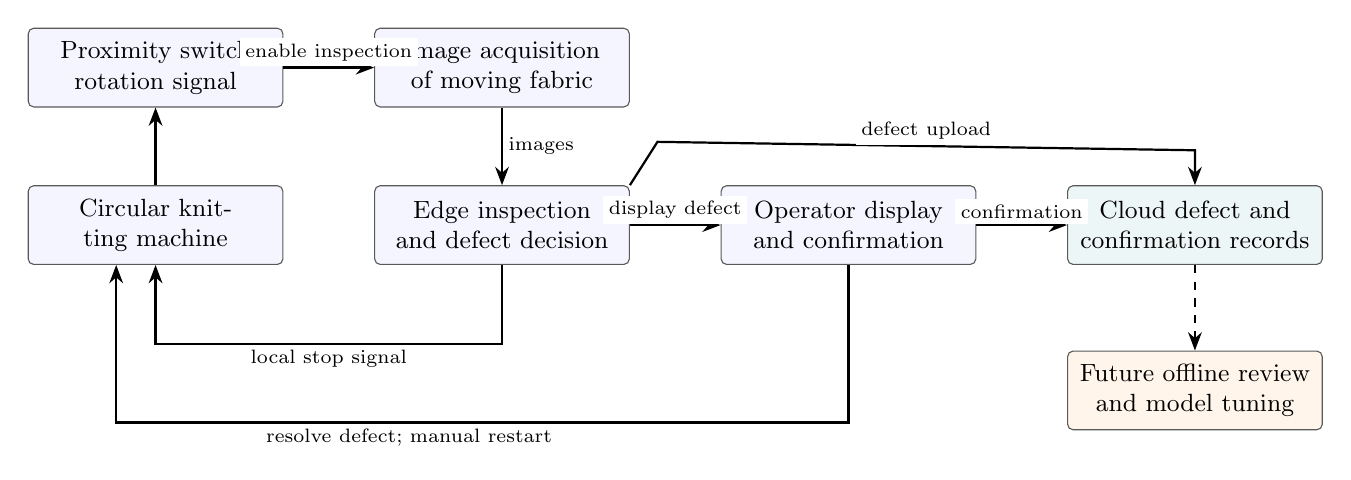
\begin{tikzpicture}[x=1cm,y=1cm,>=Stealth,
 box/.style={draw=black!65,rounded corners=2pt,align=center,minimum height=1.0cm,text width=3.0cm,font=\small,fill=blue!4},
 link/.style={->,thick},ann/.style={font=\scriptsize,align=center,fill=white,inner sep=2pt}]
 \node[box] (machine) at (0,0) {Circular knitting\ machine};
 \node[box] (edge) at (4.4,0) {Edge inspection\ and defect decision};
 \node[box] (worker) at (8.8,0) {Operator display\ and confirmation};
 \node[box,fill=teal!7] (cloud) at (13.2,0) {Cloud defect and\ confirmation records};
 \node[box] (switch) at (0,2.0) {Proximity switch\ rotation signal};
 \node[box] (camera) at (4.4,2.0) {Image acquisition\ of moving fabric};
 \node[box,fill=orange!8] (review) at (13.2,-2.1) {Future offline review\ and model tuning};
 \draw[link] (machine) -- (switch);
 \draw[link] (switch) -- node[ann,above] {enable inspection} (camera);
 \draw[link] (camera) -- node[ann,right] {images} (edge);
 \draw[link] (edge) -- node[ann,above] {display defect} (worker);
 \draw[link] (worker) -- node[ann,above] {confirmation} (cloud);
 \draw[link] (edge.south) -- ++(0,-1.0) -| node[ann,pos=0.25,below] {local stop signal} (machine.south);
 \draw[link] (worker.south) -- ++(0,-2.0) -| node[ann,pos=0.3,below] {resolve defect; manual restart} ([xshift=-5mm]machine.south);
 \draw[link] (edge.north east) -- ++(0.35,0.55) -- node[ann,above] {defect upload} (13.2,0.95) -- (cloud.north);
 \draw[link,dashed] (cloud) -- (review);
\end{tikzpicture}
}
\caption{Closed-loop inspection workflow for the circular knitting machine. Solid arrows describe the implemented production sequence provided for this study. The dashed cloud-to-review arrow represents offline data curation and later model tuning; it is not an online automatic-update claim. Hardware-specific timing and interlock details are intentionally not inferred and should be added from site measurements before submission.}
\label{fig:system}
\end{figure*}

\begin{figure*}[!t]
\centering
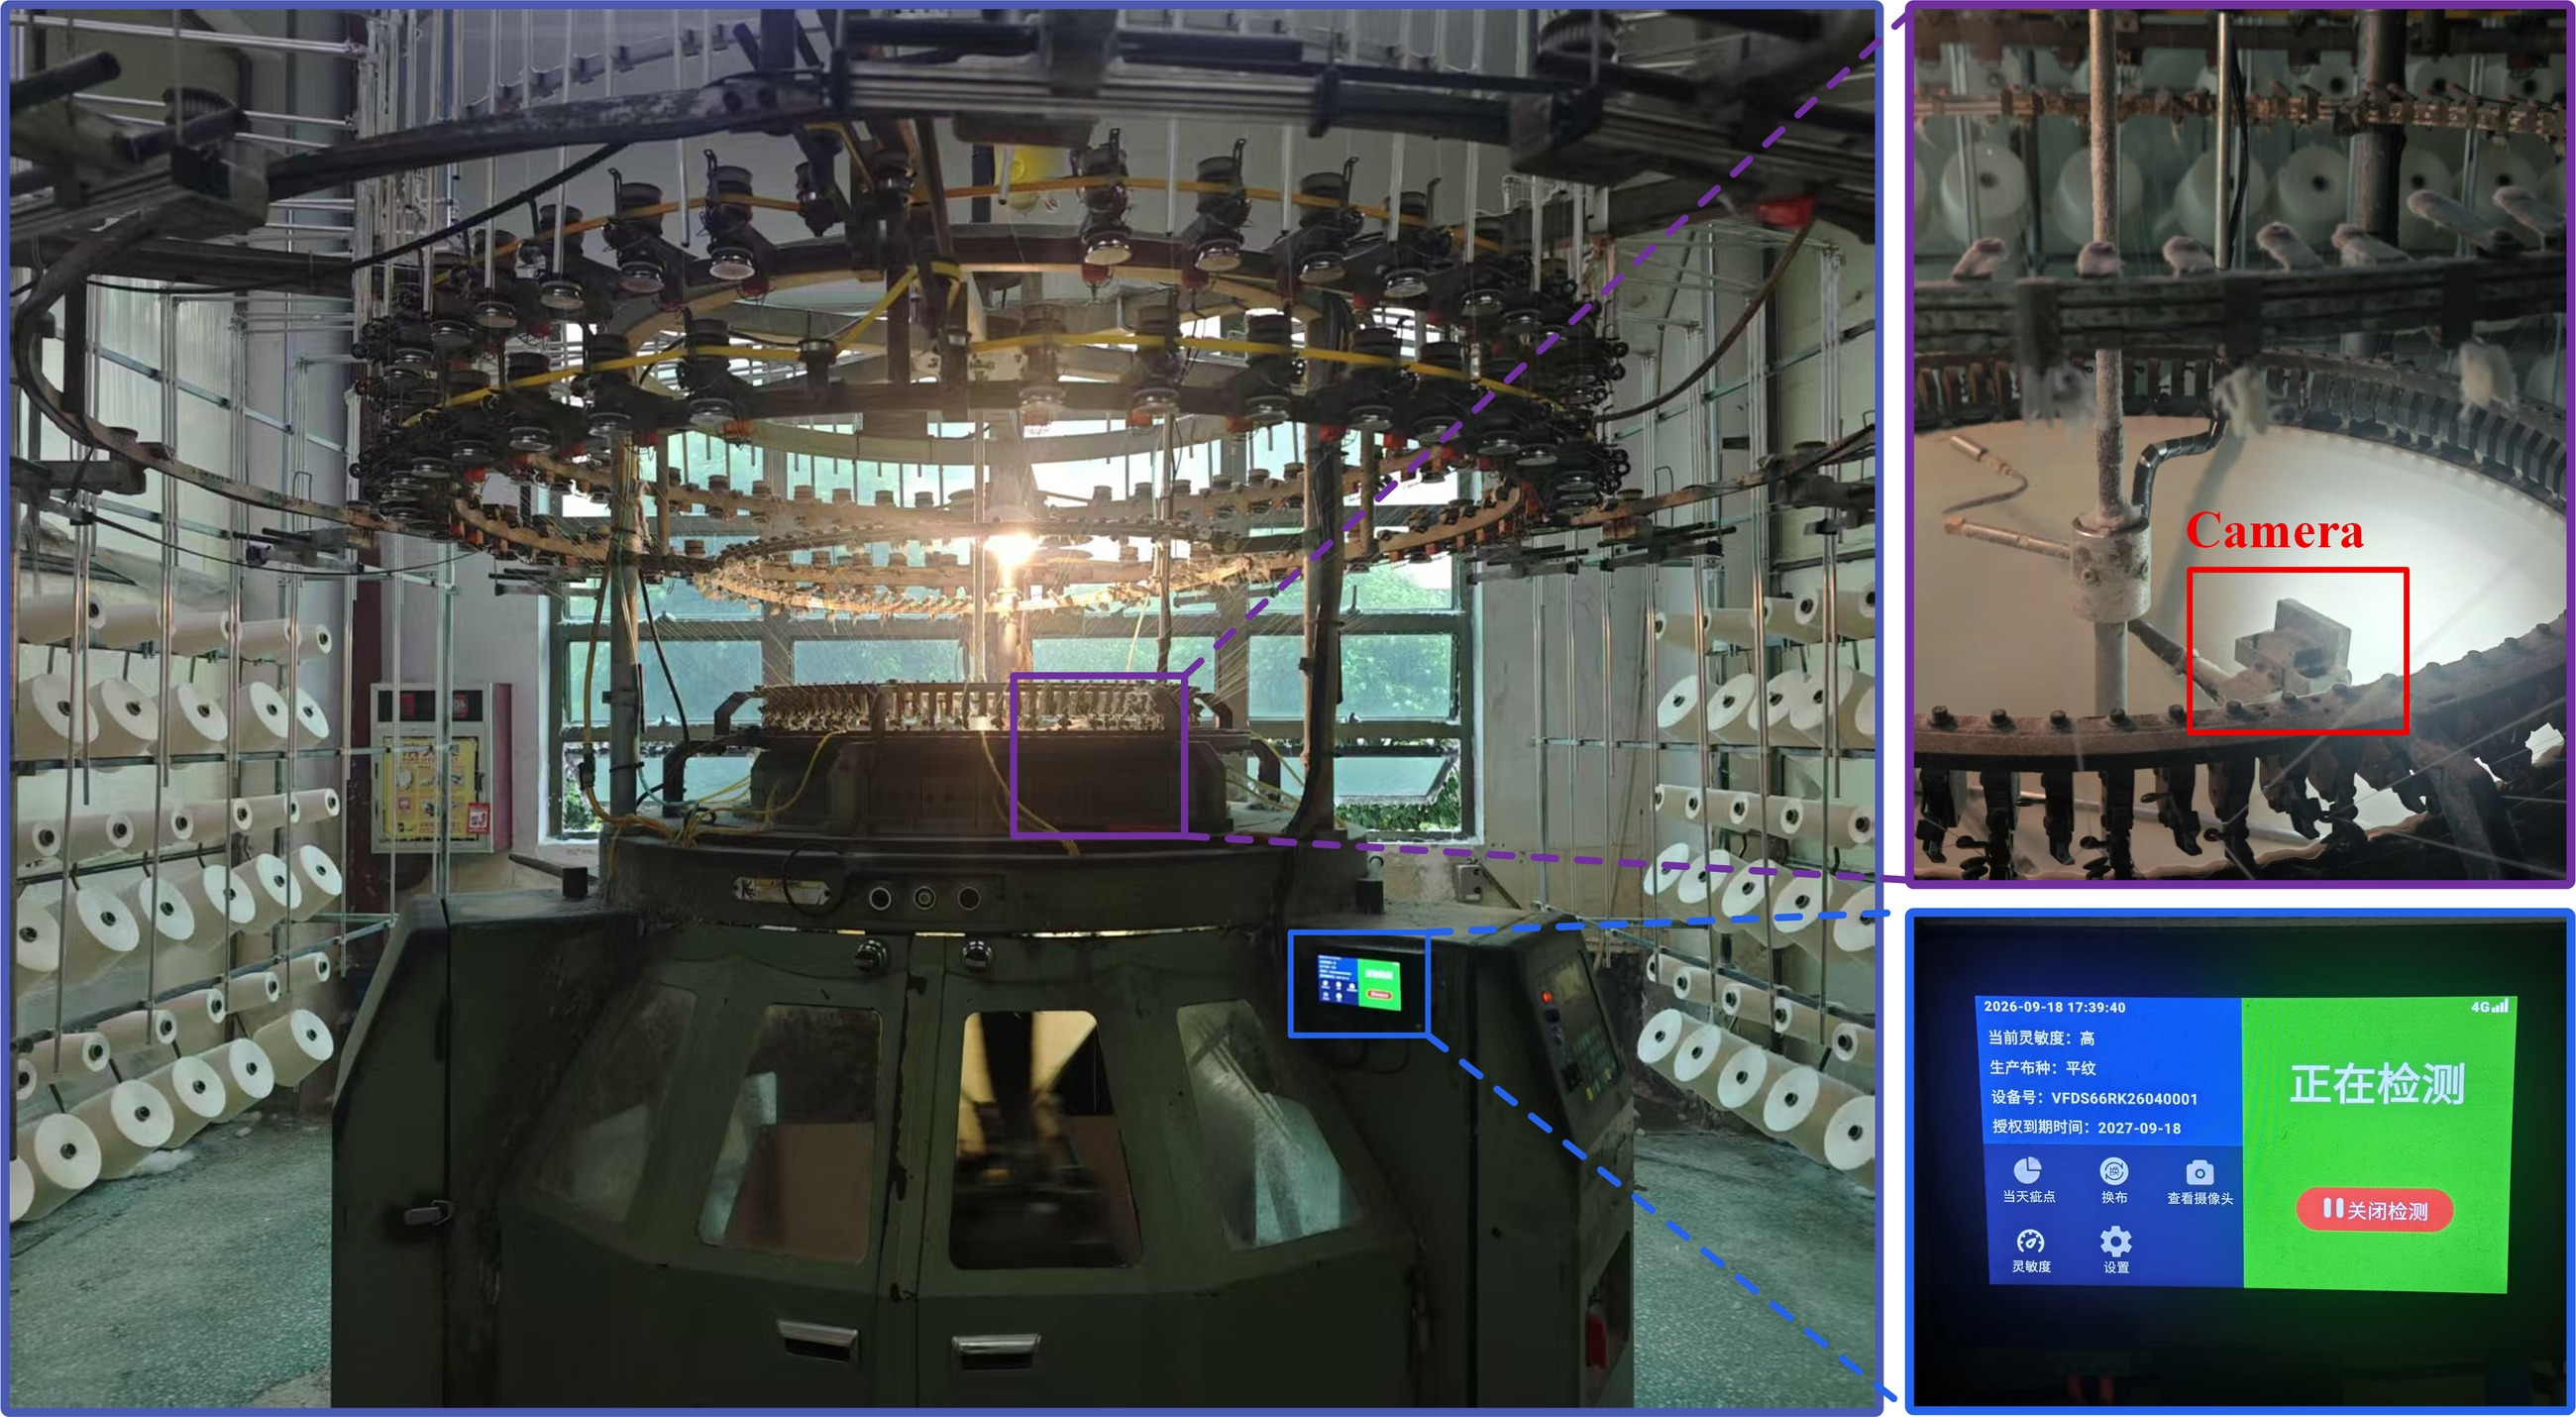
\includegraphics[width=\textwidth]{site_print.jpg}
\caption{Actual production-line installation on the circular knitting machine. The upper inset highlights the camera location; the lower inset shows the edge-side touch display while inspection is active. Colored callouts and insets are retained from the installation record.}
\label{fig:site}
\end{figure*}

The design follows the edge-intelligence principle that time-sensitive perception and action remain near the physical process, while selected evidence can be retained centrally. Related IoT work combines local detection with a cloud or digital representation for broader inspection data management \cite{saleh2025pothole}. Here, the control consequence is more direct: the event is escalated to a worker, not accepted as a final autonomous verdict. This provides a pragmatic route for handling rare defects and avoiding silent model drift.

\subsection{Operational Boundaries}
The workflow separates three decisions: (i) whether machine rotation enables inspection, (ii) whether the detector produces a candidate defect, and (iii) whether an operator confirms and disposes of the event. The reported recognition experiments validate only the second decision on a held-out image split. Actual acquisition-to-stop latency, machine stop distance, false-stop rate on defect-free fabric, availability of the control interface, and the operator-confirmation rate require site measurements and are therefore not fabricated in this draft. These measurements are specified in the accompanying material checklist.

\section{DACP-Net}
\subsection{Overview}
\model is built from the YOLOv8n detector \cite{ultralytics2023}. As shown in Fig.~\ref{fig:network}, the backbone retains the original resolution hierarchy, but replaces the C2f output refinement at four stages with C2f--WWTE. In the head, the two top-down nearest-neighbor upsampling operations are replaced with LTFR. The standard concatenation, C2f fusion, bottom-up path, and three-scale detection head are retained. The detection scales are $P_3$, $P_4$, and $P_5$, corresponding to $80\times80$, $40\times40$, and $20\times20$ feature maps for a $640\times640$ input.

\begin{figure*}[!t]
\centering
\resizebox{0.94\textwidth}{!}{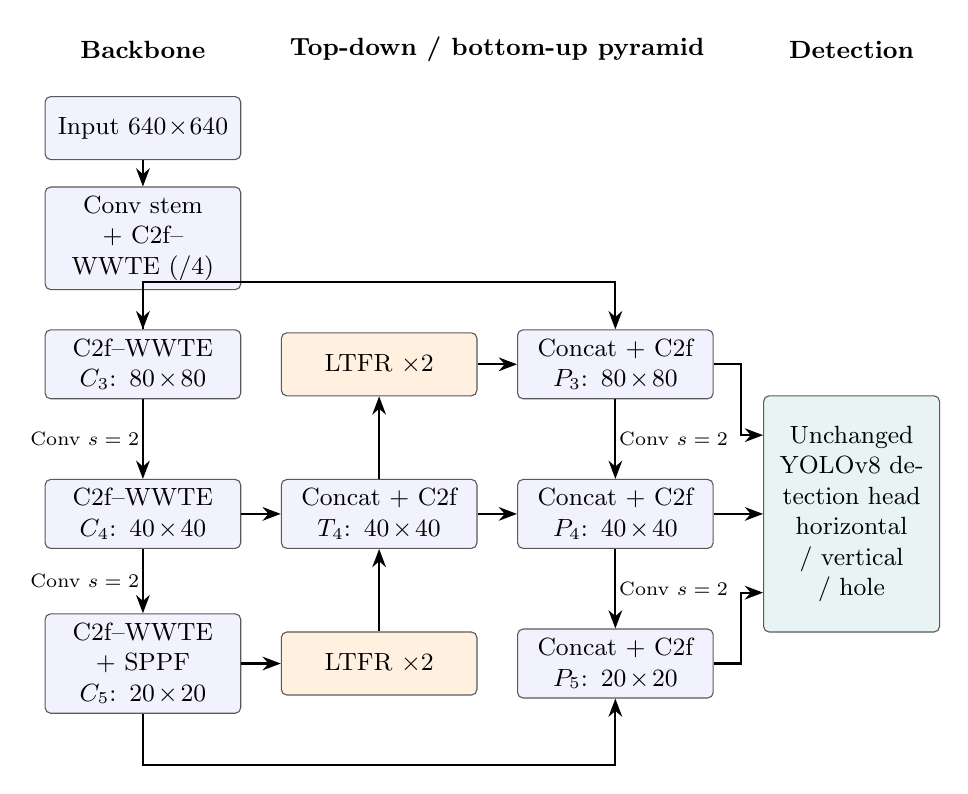
\begin{tikzpicture}[x=1cm,y=1cm,>=Stealth,
 b/.style={draw=black!65,rounded corners=2pt,align=center,font=\small,minimum height=0.8cm,text width=2.25cm,fill=blue!5},
 a/.style={->,thick}, l/.style={font=\scriptsize,fill=white,inner sep=1pt}]
 \node[b] (input) at (0,3) {Input $640\!\times\!640$};
 \node[b] (stem) at (0,1.6) {Conv stem +\ C2f--WWTE ($/4$)};
 \node[b] (c3) at (0,0) {C2f--WWTE\ $C_3$: $80\!\times\!80$};
 \node[b] (c4) at (0,-1.9) {C2f--WWTE\ $C_4$: $40\!\times\!40$};
 \node[b] (c5) at (0,-3.8) {C2f--WWTE + SPPF\ $C_5$: $20\!\times\!20$};
 \node[b,fill=orange!12] (u4) at (3.0,-3.8) {LTFR $\times2$};
 \node[b] (t4) at (3.0,-1.9) {Concat + C2f\ $T_4$: $40\!\times\!40$};
 \node[b,fill=orange!12] (u3) at (3.0,0) {LTFR $\times2$};
 \node[b] (p3) at (6,0) {Concat + C2f\ $P_3$: $80\!\times\!80$};
 \node[b] (p4) at (6,-1.9) {Concat + C2f\ $P_4$: $40\!\times\!40$};
 \node[b] (p5) at (6,-3.8) {Concat + C2f\ $P_5$: $20\!\times\!20$};
 \node[b,fill=teal!9,text width=2.0cm,minimum height=3cm] (head) at (9,-1.9) {Unchanged\ YOLOv8\ detection head\\ horizontal / vertical / hole};
 \draw[a] (input)--(stem); \draw[a] (stem)--(c3);
 \draw[a] (c3)--node[l,left] {Conv $s=2$}(c4);
 \draw[a] (c4)--node[l,left] {Conv $s=2$}(c5);
 \draw[a] (c5)--(u4); \draw[a] (u4)--(t4); \draw[a] (c4)--(t4);
 \draw[a] (t4)--(u3); \draw[a] (u3)--(p3);
 \draw[a] (c3.north) -- ++(0,0.6) -| (p3.north);
 \draw[a] (p3)--node[l,right] {Conv $s=2$}(p4);
 \draw[a] (t4)--(p4);
 \draw[a] (p4)--node[l,right] {Conv $s=2$}(p5);
 \draw[a] (c5.south) -- ++(0,-0.65) -| (p5.south);
 \draw[a] (p3.east) -- ++(.35,0) |- ([yshift=10mm]head.west);
 \draw[a] (p4.east)--(head.west);
 \draw[a] (p5.east) -- ++(.35,0) |- ([yshift=-10mm]head.west);
 \node[font=\small\bfseries] at (0,4) {Backbone};
 \node[font=\small\bfseries] at (4.5,4) {Top-down / bottom-up pyramid};
 \node[font=\small\bfseries] at (9,4) {Detection};
\end{tikzpicture}
}
\caption{Architecture of \model. C2f--WWTE replaces the four C2f refinement outputs in the backbone. LTFR replaces only the two top-down upsampling operations; the bottom-up fusion and prediction head follow YOLOv8n.}
\label{fig:network}
\end{figure*}

\subsection{Warp--Weft Texture Encoding}
The term ``warp--weft'' is retained as the internal WWTE name because it denotes two orthogonal texture directions. In this circular-knit application, it does \emph{not} imply that the fabric is woven; operationally, the branches are interpreted as horizontal and vertical texture encoders. For a C2f output $X\in\mathbb{R}^{C\times H\times W}$, WWTE applies depthwise horizontal, vertical, and local branches and then fuses them:
\begin{equation}
F(X)=\phi\left([\operatorname{DW}_{1\times7}(X),\operatorname{DW}_{7\times1}(X),\operatorname{DW}_{3\times3}(X)]\right),
\label{eq:wwte}
\end{equation}
where $[\cdot]$ denotes channel concatenation and $\phi$ is a $1\times1$ convolution with normalization and activation. Because input and output channels match in the present implementation, the module uses residual fusion:
\begin{equation}
Y=X+F(X).
\label{eq:wwte-residual}
\end{equation}
The long $1\times7$ and $7\times1$ depthwise kernels make the representation responsive to thin texture discontinuities in either image direction, while the $3\times3$ path supplies local texture evidence. The design is related to, but not equivalent to, asymmetric convolution blocks \cite{ding2019acnet}: it uses depthwise directional paths and a learned concatenation fusion within the existing C2f structure.

\subsection{Local Texture-Guided Feature Reassembly}
Fixed nearest-neighbor upsampling copies a source value to each new location and cannot adapt to nearby texture. LTFR uses the content-aware reassembly principle of CARAFE \cite{wang2019carafe} at each of the two top-down transitions. Given input $X$, a $1\times1$ compression produces $H$ channels, with $H=\max(C/4,16)$. A $3\times3$ encoder produces $s^2k^2$ kernel logits, where the scale factor is $s=2$ and $k=5$. Pixel shuffle followed by softmax yields a location-specific $5\times5$ kernel $K_{i,j}$:
\begin{equation}
K_{i,j}=\operatorname{softmax}\left(\operatorname{PS}\left(E_{3\times3}(E_{1\times1}(X))\right)_{i,j}\right).
\label{eq:ltfr-kernel}
\end{equation}
For each output position, a $5\times5$ neighborhood $\mathcal{N}_{i,j}(X)$ is unfolded from $X$, repeated to the enlarged grid, and reassembled as
\begin{equation}
Y_{i,j}=\sum_{u=1}^{25}K_{i,j,u}\mathcal{N}_{i,j,u}(X).
\label{eq:ltfr-reassembly}
\end{equation}
Thus, the reassembly weights adapt to local texture rather than being spatially shared. Fig.~\ref{fig:modules} details both modules.

\begin{figure*}[!t]
\centering
\resizebox{0.88\textwidth}{!}{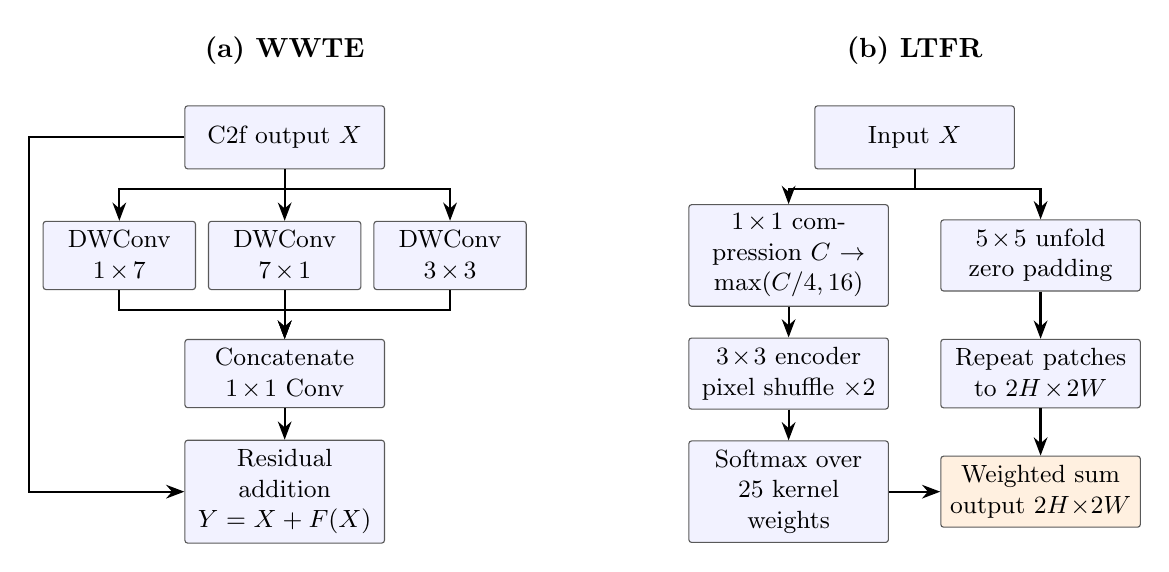
\begin{tikzpicture}[x=1cm,y=1cm,>=Stealth,
 b/.style={draw=black!65,rounded corners=1pt,font=\small,align=center,minimum height=.8cm,text width=2.3cm,fill=blue!5},
 a/.style={->,thick},l/.style={font=\scriptsize,fill=white,inner sep=1pt}]
 \node[font=\bfseries] at (0,3.8) {(a) WWTE};
 \node[b] (x) at (0,2.7) {C2f output $X$};
 \node[b,text width=1.7cm] (h) at (-2.1,1.2) {DWConv $1\!\times\!7$};
 \node[b,text width=1.7cm] (v) at (0,1.2) {DWConv $7\!\times\!1$};
 \node[b,text width=1.7cm] (d) at (2.1,1.2) {DWConv $3\!\times\!3$};
 \node[b] (cat) at (0,-.3) {Concatenate\ $1\!\times\!1$ Conv};
 \node[b] (sum) at (0,-1.8) {Residual addition\ $Y=X+F(X)$};
 \draw[a] (x.south) -- ++(0,-.25) -| (h.north);
 \draw[a] (x)--(v);
 \draw[a] (x.south) -- ++(0,-.25) -| (d.north);
 \draw[a] (h.south) -- ++(0,-.25) -| (cat.north);
 \draw[a] (v)--(cat);
 \draw[a] (d.south) -- ++(0,-.25) -| (cat.north);
 \draw[a] (cat)--(sum);
 \draw[a] (x.west) -- (-3.25,2.7) |- (sum.west);
 \node[font=\bfseries] at (8,3.8) {(b) LTFR};
 \node[b] (lx) at (8,2.7) {Input $X$};
 \node[b] (compress) at (6.4,1.2) {$1\!\times\!1$ compression\ $C\to\max(C/4,16)$};
 \node[b] (kernel) at (6.4,-.3) {$3\!\times\!3$ encoder\ pixel shuffle $\times2$};
 \node[b] (sm) at (6.4,-1.8) {Softmax over\ 25 kernel weights};
 \node[b] (patch) at (9.6,1.2) {$5\!\times\!5$ unfold\ zero padding};
 \node[b] (repeat) at (9.6,-.3) {Repeat patches\ to $2H\!\times\!2W$};
 \node[b,fill=orange!12] (out) at (9.6,-1.8) {Weighted sum\ output $2H\!\times\!2W$};
 \draw[a] (lx.south) -- ++(0,-.25) -| (compress.north);
 \draw[a] (lx.south) -- ++(0,-.25) -| (patch.north);
 \draw[a] (compress)--(kernel); \draw[a] (kernel)--(sm);
 \draw[a] (patch)--(repeat); \draw[a] (repeat)--(out);
 \draw[a] (sm)--(out);
\end{tikzpicture}
}
\caption{Internal structures of (a) WWTE and (b) LTFR. WWTE uses three depthwise branches and residual fusion. LTFR is a compact CARAFE-style $2\times$ operator: it predicts location-specific $5\times5$ kernels and reassembles aligned local feature patches.}
\label{fig:modules}
\end{figure*}

\section{Experimental Protocol}
\subsection{Dataset}
The data were collected from a real textile production line. The three object categories are \emph{horizontal defect}, \emph{vertical defect}, and \emph{hole}. Table~\ref{tab:data} summarizes the provided image-level split and instance counts. The test set contains 81 images with 91 labeled defects. This small, imbalanced test set makes every retained result useful for engineering comparison but is insufficient by itself to support a broad generalization claim. A future submission should state whether the split is grouped by production roll, machine, material, or time interval, and should add an independent production-period test set if available.

\begin{table}[!t]
\caption{Dataset split supplied for the current draft.}
\label{tab:data}
\centering
\footnotesize
\begin{tabular}{lrrrrr}
\toprule
Split & Images & Instances & Horizontal & Vertical & Hole \\
\midrule
Train & 282 & 329 & 174 & 75 & 80 \\
Validation & 40 & 48 & 24 & 13 & 11 \\
Test & 81 & 91 & 60 & 12 & 19 \\
\bottomrule
\end{tabular}
\end{table}

\subsection{Training and Evaluation}
All models use the available pretrained initialization and $640\times640$ input. For the Ultralytics experiments, the retained configuration uses 300 maximum epochs, patience 80, batch size 16, automatic optimizer selection, and the framework's standard geometric and photometric augmentations; the DACP-Net checkpoint is initialized from \texttt{yolov8n.pt}. Evaluation is conducted on the held-out test split with a maximum of 16 detections per image. We report COCO-style AP averaged over IoU thresholds 0.50:0.95 and AP50. AP values are written as percentages.

The comparison table contains the latest retained checkpoint output for each model, rather than a mean over matched random seeds. FLOPs and parameter counts are reported at $[1,3,640,640]$. The values are suitable for a coarse efficiency comparison, but cross-framework FLOP accounting can omit unsupported operators; no cross-framework latency claim is made. DETR, Deformable DETR, Faster R-CNN, and RT-DETRv2 follow their respective repositories and pretrained backbones \cite{carion2020detr,zhu2021deformable,ren2015faster,lv2024rtdetrv2}.

\section{Results and Discussion}
\subsection{Comparison With Detectors}
Table~\ref{tab:comparison} compares \model with the retained baselines. \model achieves 66.3\% AP and 96.9\% AP50. Relative to its direct YOLOv8n baseline, AP improves by 7.0 points and AP50 by 2.8 points for 0.38 M additional parameters and 0.8 G additional FLOPs. Among the compact YOLO variants evaluated here, \model has the highest AP. RT-DETR-R18 obtains 67.7\% AP, 1.4 points higher than \model, but requires 20.09 M parameters and 60.72 G FLOPs. This is a useful trade-off rather than a claim that \model dominates every detector.

\begin{table*}[!t]
\caption{Test-set comparison on 81 images and 91 instances. AP is COCO AP@[.50:.95]. All values are percentages except parameters and FLOPs.}
\label{tab:comparison}
\centering
\small
\begin{tabular}{lrrrr}
\toprule
Model & Params (M) & FLOPs (G) & AP50 (\%) & AP (\%) \\
\midrule
YOLOv5n$^\dagger$ & 2.50 & 7.10 & 93.1 & 58.4 \\
YOLOv8n & 3.01 & 8.10 & 94.1 & 59.3 \\
YOLO11n & 2.58 & 6.40 & 95.0 & 59.6 \\
YOLO12n & 2.56 & 7.30 & 94.3 & 60.9 \\
YOLO26n & 2.38 & 5.30 & 96.5 & 61.4 \\
RT-DETR-R18 & 20.09 & 60.72 & 95.2 & \textbf{67.7} \\
DETR-R50 & 41.28 & 77.25 & 96.4 & 53.6 \\
Deformable DETR-R50 & 39.82 & 158.66 & 96.8 & 64.3 \\
Faster R-CNN-R50 & 41.13 & 181.45 & 96.1 & 64.7 \\
\midrule
\model & 3.39 & 8.90 & \textbf{96.9} & 66.3 \\
\bottomrule
\multicolumn{5}{l}{\footnotesize $^\dagger$The retained YOLOv5n checkpoint is the legacy YOLOv5n architecture, not the Ultralytics YOLOv5u variant.}
\end{tabular}
\end{table*}

Fig.~\ref{fig:tradeoff} visualizes the parameter- and operation-accuracy trade-off without shifting any data coordinates. The position of \model in the low-parameter region is consistent with the tabulated result. Because the horizontal axes are logarithmic, the visual is intended to show scale rather than imply a linear performance-efficiency relationship.

\begin{figure*}[!t]
\centering
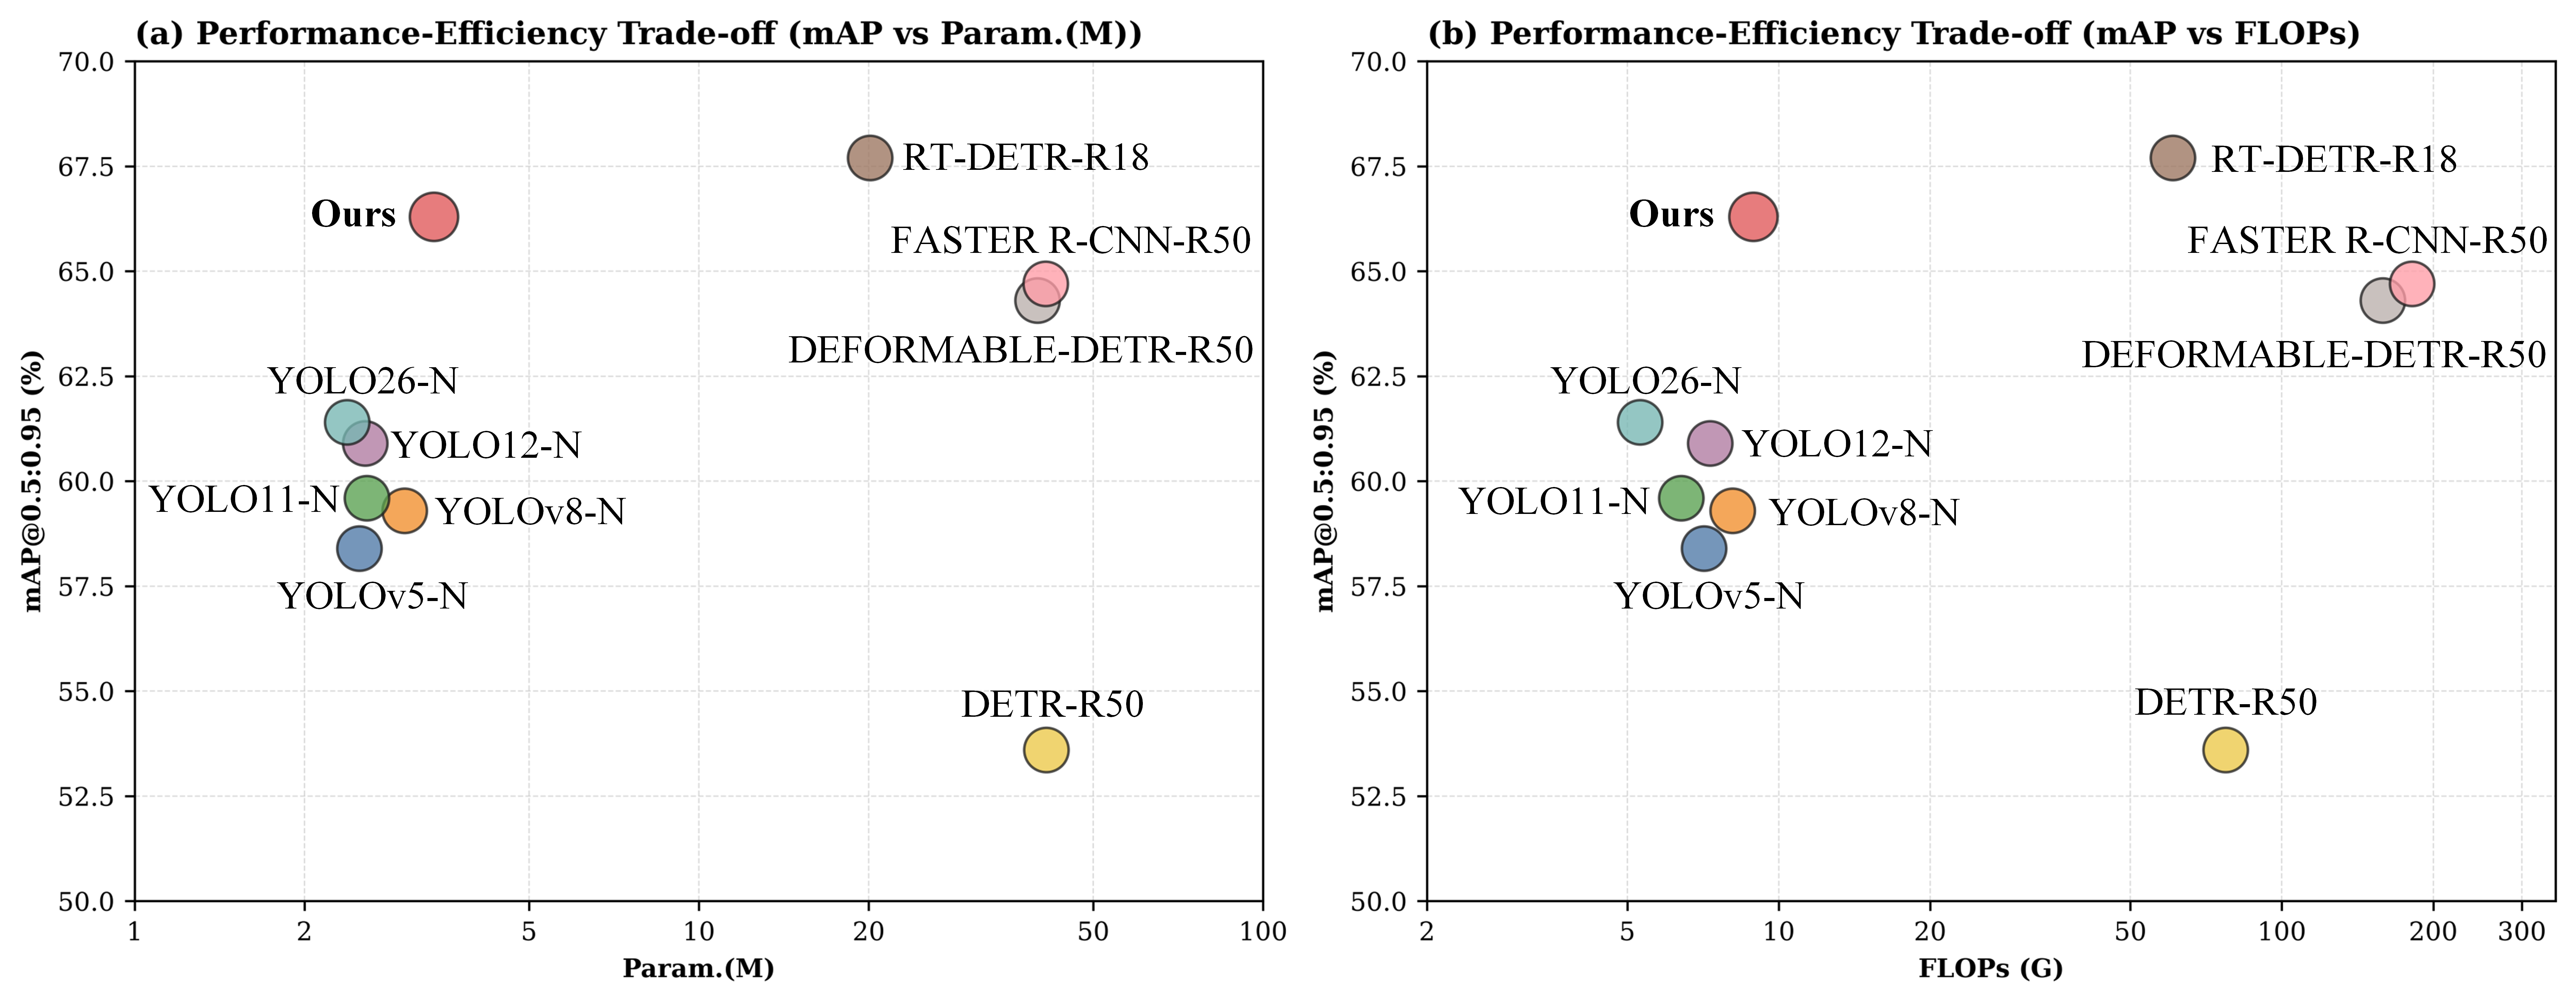
\includegraphics[width=.97\textwidth]{efficiency.png}
\caption{Accuracy-efficiency trade-off of the retained test results. Both horizontal axes use a logarithmic scale. Marker coordinates are the exact values in Table~\ref{tab:comparison}; the plot does not contain manual coordinate compression.}
\label{fig:tradeoff}
\end{figure*}

\subsection{Ablation}
Table~\ref{tab:ablation} isolates the two modifications with the same YOLOv8n family. WWTE contributes the larger retained isolated improvement (+4.8 AP), while LTFR contributes +1.6 AP. Combining both gives 66.3\% AP, which is 0.6 points above the arithmetic sum of the isolated gains. This suggests that the directional representation and adaptive reassembly are complementary: WWTE supplies direction-specific texture cues, whereas LTFR transfers them through the top-down path. However, the four retained checkpoints are not matched-seed repetitions, so this interpretation is preliminary. Before submission, this table should be rerun with identical seeds, training budget, and reporting of mean and standard deviation.

\begin{table}[!t]
\caption{Ablation on the test split. The current retained runs use the same architecture family and training recipe, but are not matched-seed repetitions.}
\label{tab:ablation}
\centering
\footnotesize
\begin{tabular}{lccrrrr}
\toprule
Variant & WWTE & LTFR & Params & FLOPs & AP50 & AP \\
\midrule
YOLOv8n & -- & -- & 3.01 & 8.1 & 94.1 & 59.3 \\
+ WWTE & \checkmark & -- & 3.28 & 8.8 & 94.2 & 64.1 \\
+ LTFR & -- & \checkmark & 3.11 & 8.2 & 94.3 & 60.9 \\
\model & \checkmark & \checkmark & 3.39 & 8.9 & 96.9 & 66.3 \\
\bottomrule
\end{tabular}
\end{table}

\subsection{Per-Class and Qualitative Results}
The \model checkpoint obtains 61.7\%, 73.8\%, and 63.4\% AP for horizontal defects, vertical defects, and holes, respectively. The notably high vertical-defect AP should be interpreted with care because the test category has only 12 instances. Fig.~\ref{fig:qualitative} presents seven selected images and the available standardized renderings. The visual comparison is illustrative rather than a replacement for the full quantitative test set. It is particularly useful for examining thin vertical defects, long horizontal defects, and the hole class against repetitive background texture.

\begin{figure*}[!t]
\centering
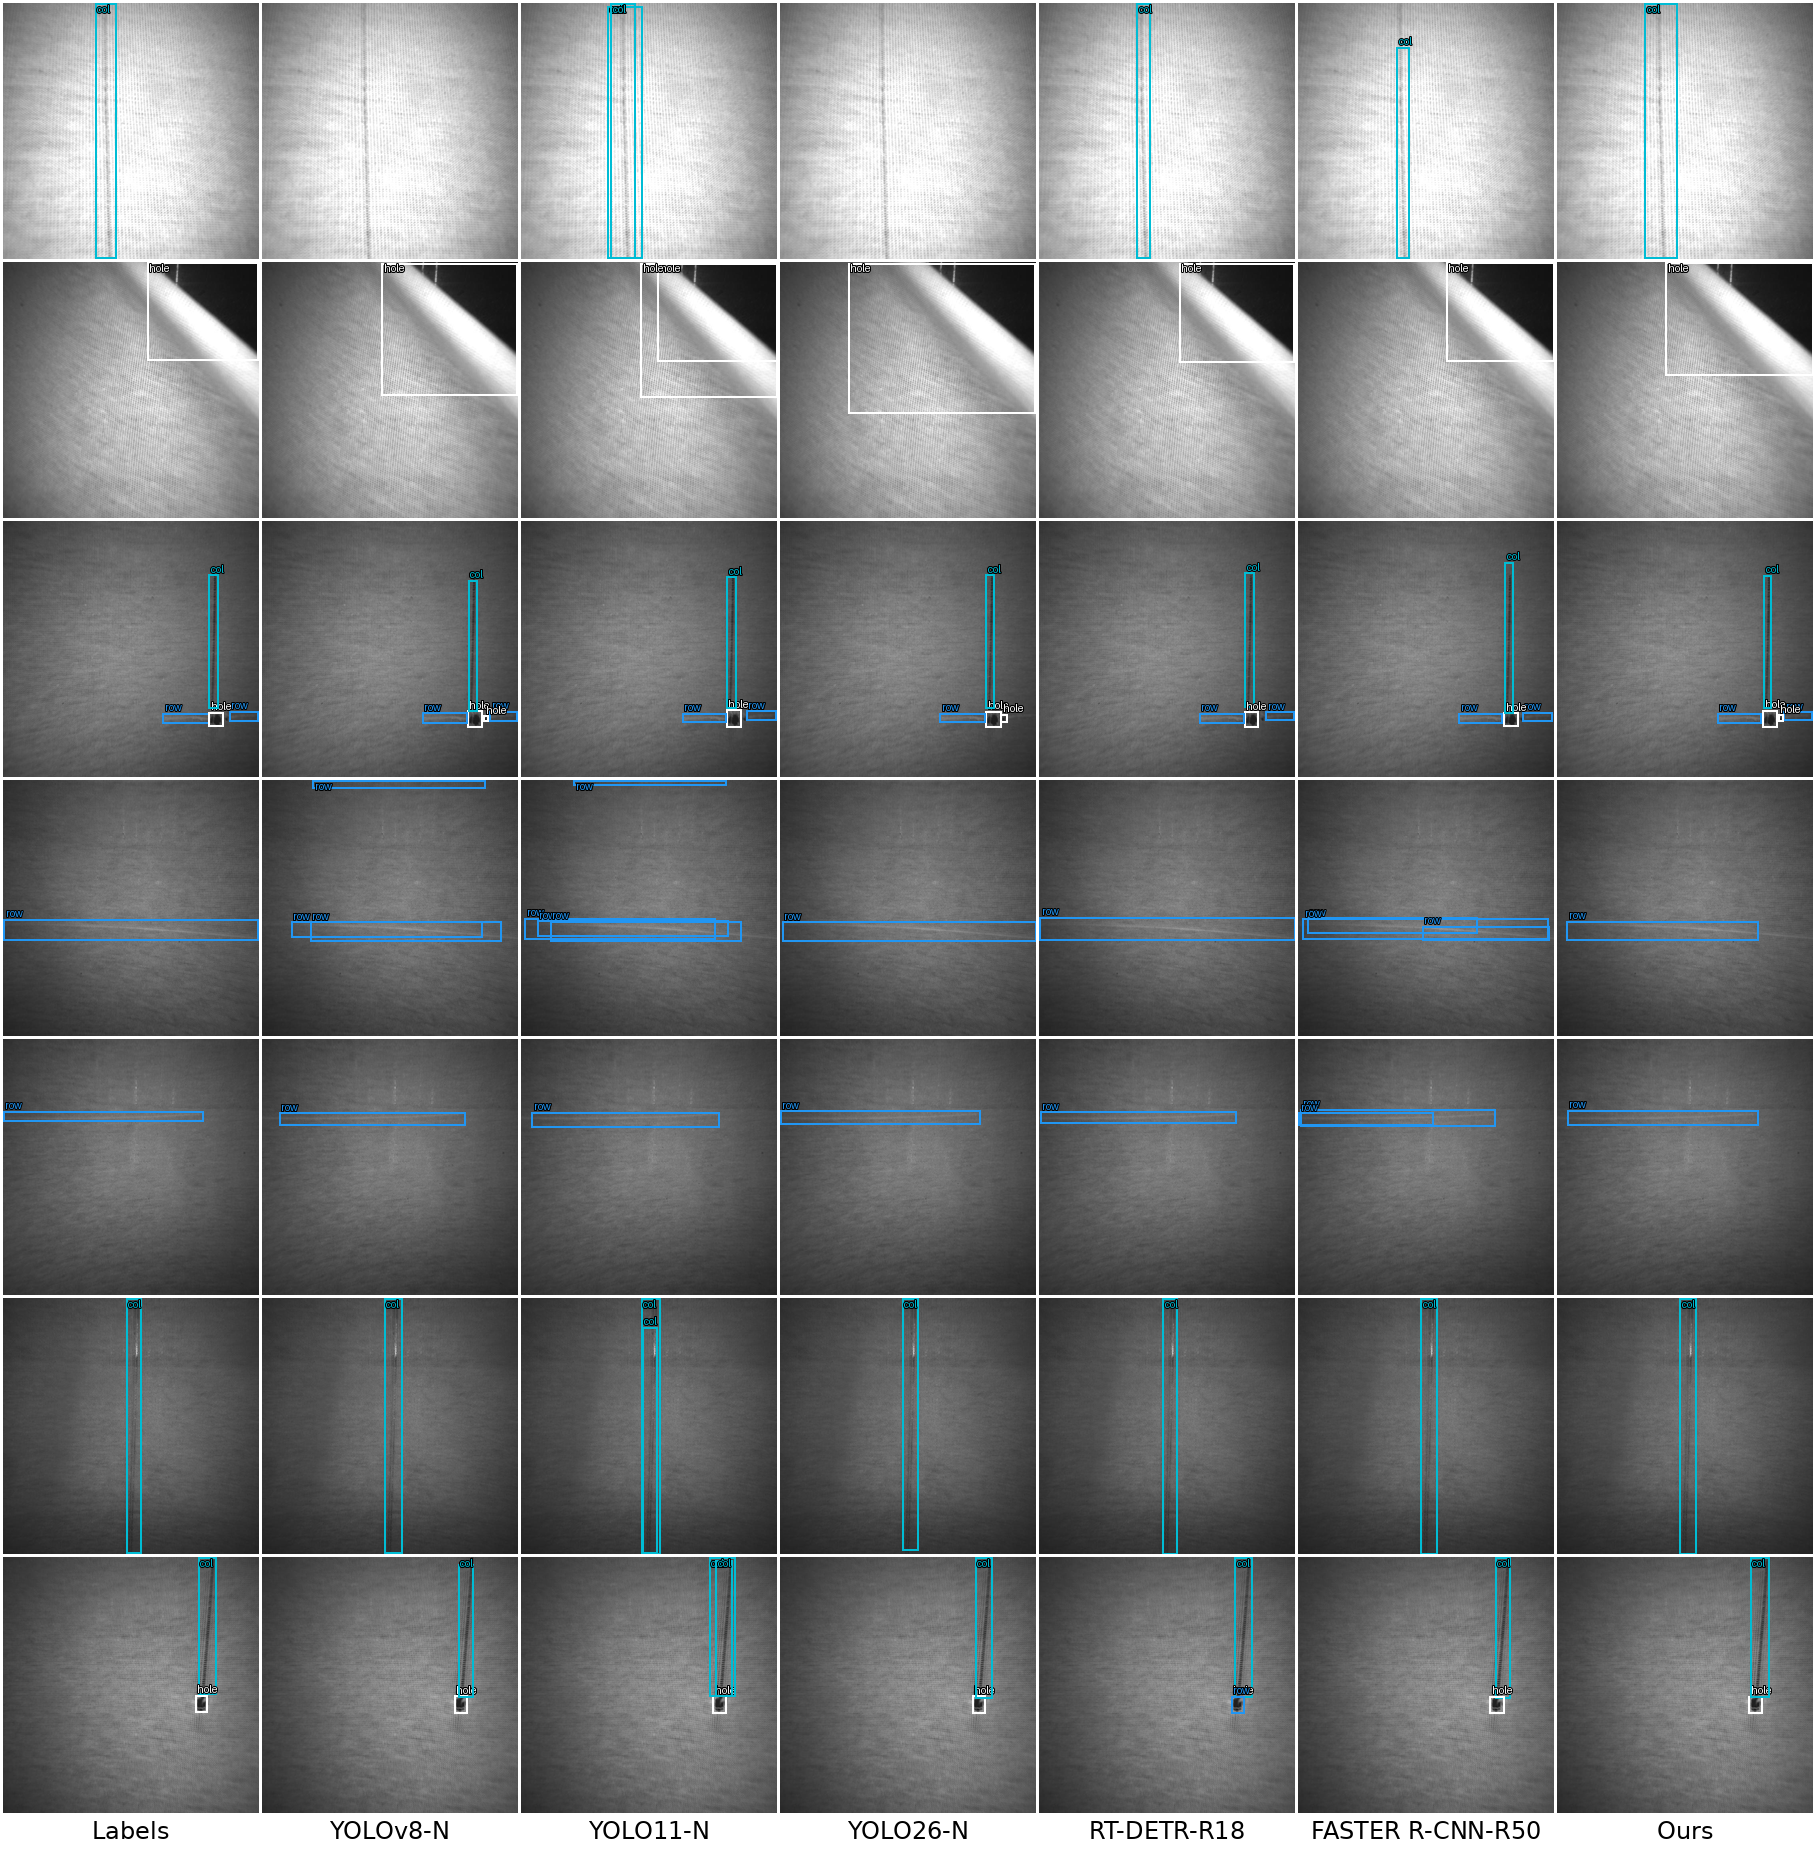
\includegraphics[width=\textwidth]{qualitative_existing.png}
\caption{Qualitative comparison on selected test images. Columns are labels, YOLOv8n, YOLO11n, YOLO26n, RT-DETR-R18, Faster R-CNN-R50, and \model. The figure uses a common renderer for visual consistency; it should be updated after finalizing the exact sample-selection protocol and display confidence threshold.}
\label{fig:qualitative}
\end{figure*}

\subsection{Limitations and Submission-Ready Validation}
The present evidence supports a promising lightweight detector on a real production-line image set, but it does not yet establish production reliability. First, the test split is small and category-imbalanced. Second, a direct comparison must use aligned training seeds and preferably report mean and standard deviation. Third, FLOPs are not a substitute for end-to-end edge latency, especially when image capture, preprocessing, postprocessing, control communication, and physical stopping are part of the operational loop. Finally, the operator's confirmation records are intended to support curated offline updates; their actual acceptance rate and impact on subsequent retraining have not yet been measured. These points define a concrete validation plan, rather than weaknesses that should be concealed.

\section{Conclusion}
This work presents a closed-loop framework for defect inspection on a circular knitting machine and \model, a compact direction- and content-adaptive detector. The workflow couples rotation-aware edge inspection, local stop signaling, human confirmation, and cloud-side record retention. The detector combines WWTE for horizontal, vertical, and local knitted-texture encoding with LTFR for adaptive feature-pyramid reconstruction. On the retained test split, \model improves YOLOv8n from 59.3\% to 66.3\% AP at 3.39 M parameters and 8.9 G FLOPs. The next step is not merely more offline accuracy: it is a disciplined site evaluation of sensing-to-stop latency, false-stop behavior, confirmation outcomes, and grouped generalization across production conditions.

\bibliographystyle{IEEEtran}
\bibliography{references}

\end{document}
